\documentclass[letterpaper,12pt]{article}
\usepackage{tabularx,amsmath,graphicx}
\usepackage[margin=1in,letterpaper]{geometry}
\usepackage{cite}
\usepackage[final]{hyperref}
\hypersetup{
colorlinks=true,
linkcolor=blue,
citecolor=blue,
filecolor=magenta,
urlcolor=blue         
}
\begin{document}
\title{Lab 1: Prelab}
\author{Joshua Emele $<$jemele@acm.org$>$}
\maketitle

\section{Theory Problems}

\begin{figure}[ht] 
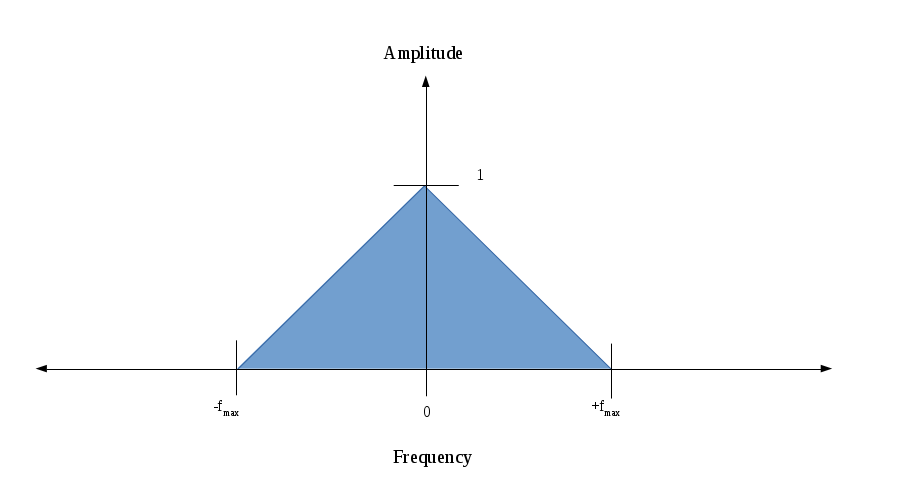
\includegraphics[width=1.0\columnwidth]{prelab1-figure1}
\caption{
\label{fig:hw1-figure1}
{\bf Describe figure 1...
here}
}
\end{figure}

\begin{figure}[ht] 
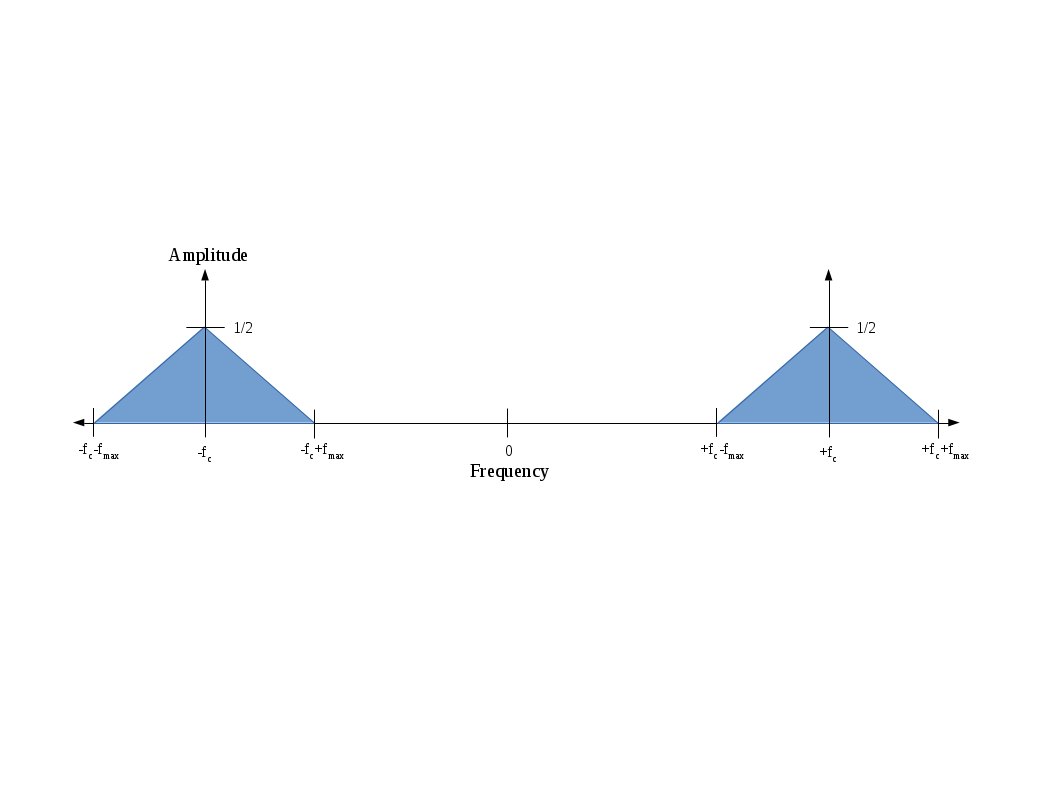
\includegraphics[width=1.0\columnwidth]{prelab1-figure1a}
\caption{
\label{fig:hw1-figure1a}
{\bf Describe figure 1a...
here}
}
\end{figure}

\begin{figure}[ht] 
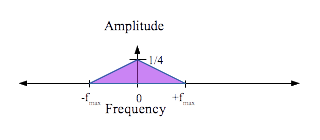
\includegraphics[width=1.0\columnwidth]{prelab1-figure1b}
\caption{
\label{fig:hw1-figure1b}
{\bf Describe figure 1b...
here}
}
\end{figure}

\begin{figure}[ht] 
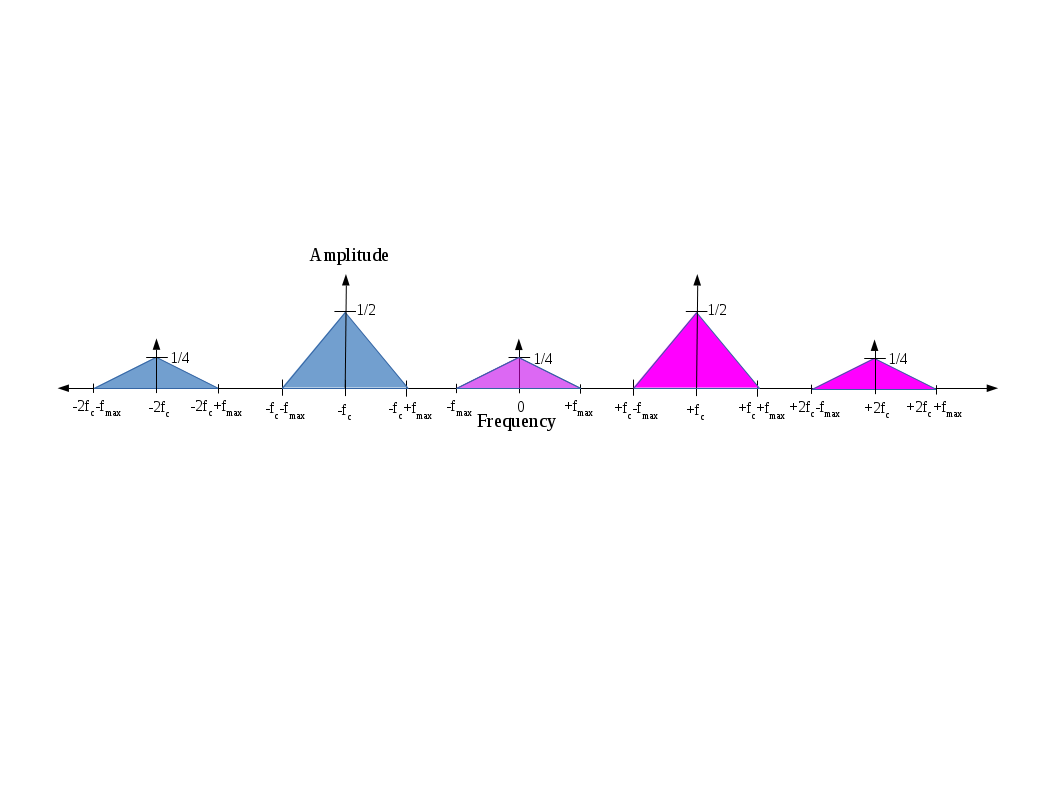
\includegraphics[width=1.0\columnwidth]{prelab1-figure2a}
\caption{
\label{fig:hw1-figure2a}
{\bf Describe  figure 2a...
here}
}
\end{figure}

\begin{figure}[ht] 
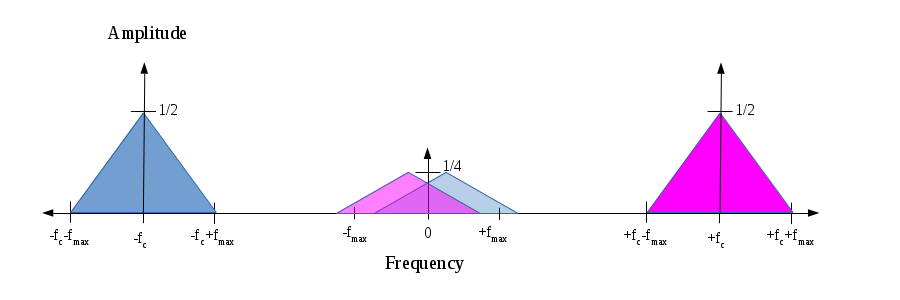
\includegraphics[width=1.0\columnwidth]{prelab1-figure2b}
\caption{
\label{fig:hw1-figure2b}
{\bf Describe  figure 2b...
here}
}
\end{figure}

\begin{figure}[ht] 
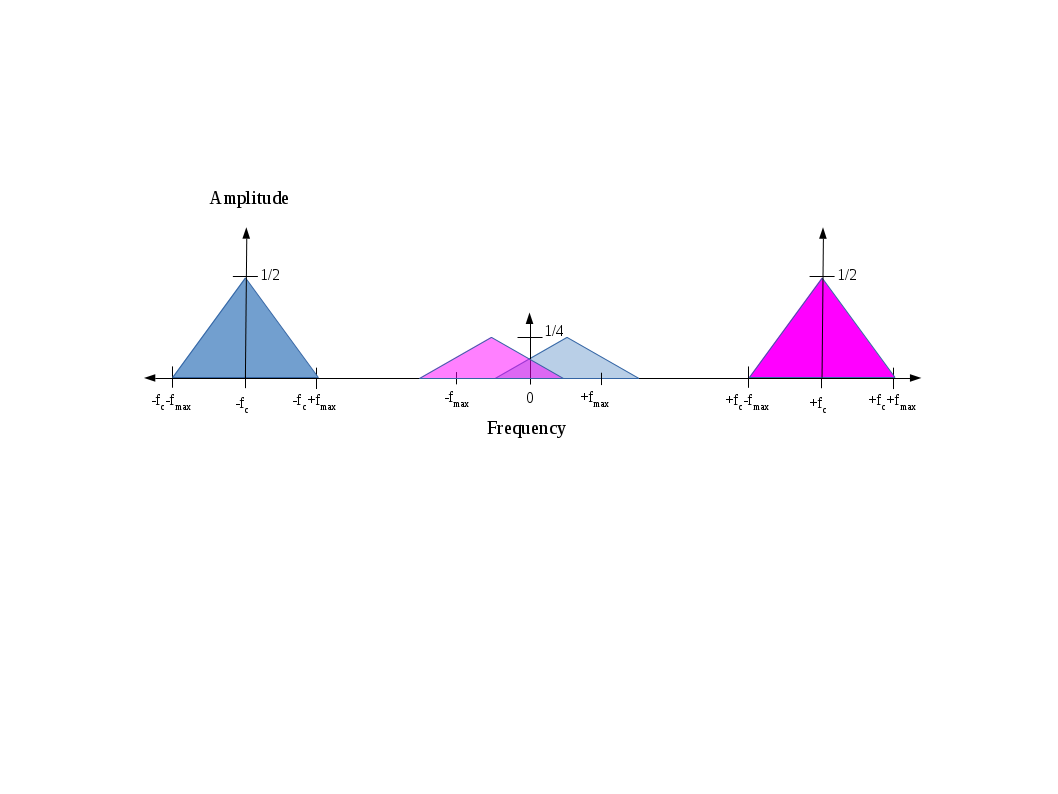
\includegraphics[width=1.0\columnwidth]{prelab1-figure2c}
\caption{
\label{fig:hw1-figure2c}
{\bf Describe  figure 2c...
here}
}
\end{figure}


\section{Matlab/Simulink Simulations}

\end{document}
